% \documentclass[handout]{beamer}
\documentclass{beamer}

\mode<presentation>
{
  \usetheme{ANLBlue}
  % \usefonttheme[onlymath]{serif}
  % \usetheme{Singapore}
  % \usetheme{Warsaw}
  % \usetheme{Malmoe}
  % \useinnertheme{circles}
  % \useoutertheme{infolines}
  % \useinnertheme{rounded}

  \setbeamercovered{transparent=20}
}

\usepackage[english]{babel}
\usepackage[latin1]{inputenc}
\usepackage{alltt,listings,multirow,ulem,siunitx}
\usepackage[absolute,overlay]{textpos}
\TPGrid{1}{1}
\usepackage{pdfpages}
\usepackage{ulem}
\usepackage{multimedia}
\usepackage{multicol}
\newcommand\hmmax{0}
\newcommand\bmmax{0}
\usepackage{bm}
\usepackage{comment}
\usepackage{subcaption}

% font definitions, try \usepackage{ae} instead of the following
% three lines if you don't like this look
\usepackage{mathptmx}
\usepackage[scaled=.90]{helvet}
% \usepackage{courier}
\usepackage[T1]{fontenc}
\usepackage{tikz}
\usetikzlibrary{decorations.pathreplacing}
\usetikzlibrary{shadows,arrows,shapes.misc,shapes.arrows,shapes.multipart,arrows,decorations.pathmorphing,backgrounds,positioning,fit,petri,calc,shadows,chains,matrix}

\newcommand\vvec{\bm v}
\newcommand\bvec{\bm b}
\newcommand\bxk{\bvec_0 \times \kappa_0 \cdot \nabla}
\newcommand\delp{\nabla_\perp}

% \usepackage{pgfpages}
% \pgfpagesuselayout{4 on 1}[a4paper,landscape,border shrink=5mm]

\usepackage{JedMacros}

\newcommand{\timeR}{t_{\mathrm{R}}}
\newcommand{\timeW}{t_{\mathrm{W}}}
\newcommand{\mglevel}{\ensuremath{\ell}}
\newcommand{\mglevelcp}{\ensuremath{\mglevel_{\mathrm{cp}}}}
\newcommand{\mglevelcoarse}{\ensuremath{\mglevel_{\mathrm{coarse}}}}
\newcommand{\mglevelfine}{\ensuremath{\mglevel_{\mathrm{fine}}}}

%solution and residual
\newcommand{\vx}{\ensuremath{x}}
\newcommand{\vc}{\ensuremath{\hat{x}}}
\newcommand{\vr}{\ensuremath{r}}
\newcommand{\vb}{\ensuremath{b}}

%operators
\newcommand{\vA}{\ensuremath{A}}
\newcommand{\vP}{\ensuremath{I_H^h}}
\newcommand{\vS}{\ensuremath{S}}
\newcommand{\vR}{\ensuremath{I_h^H}}
\newcommand{\vI}{\ensuremath{\hat I_h^H}}
\newcommand{\vV}{\ensuremath{\mathbf{V}}}
\newcommand{\vF}{\ensuremath{F}}
\newcommand{\vtau}{\ensuremath{\mathbf{\tau}}}


\title{Towards $\tau$ adaptivity \\ for lithosphere dynamics}
\subtitle{Non-smooth processes in heterogeneous media}
\author{{\bf Jed Brown} \texttt{jedbrown@mcs.anl.gov} (ANL and CU Boulder) \\
  \quad Mark Adams (LBL), Matt Knepley (UChicago), Dave May (ETH)
}

% - Use the \inst command only if there are several affiliations.
% - Keep it simple, no one is interested in your street address.
% \institute
% {
%   Mathematics and Computer Science Division \\ Argonne National Laboratory
% }

\date{SIAM Annual Meeting, Chicago, 2014-07-07 \\[1em]
This talk: \url{http://59A2.org/files/20140707-SIAMAnnual.pdf}}

% This is only inserted into the PDF information catalog. Can be left
% out.
\subject{Talks}


% If you have a file called "university-logo-filename.xxx", where xxx
% is a graphic format that can be processed by latex or pdflatex,
% resp., then you can add a logo as follows:

% \pgfdeclareimage[height=0.5cm]{university-logo}{university-logo-filename}
% \logo{\pgfuseimage{university-logo}}



% Delete this, if you do not want the table of contents to pop up at
% the beginning of each subsection:
% \AtBeginSubsection[]
% {
% \begin{frame}<beamer>
%   \frametitle{Outline}
%   \tableofcontents[currentsection,currentsubsection]
% \end{frame}
% }

% \AtBeginSection[]
% {
%   \begin{frame}<beamer>
%     \frametitle{Outline}
%     \tableofcontents[currentsection]
%   \end{frame}
% }

% If you wish to uncover everything in a step-wise fashion, uncomment
% the following command:

% \beamerdefaultoverlayspecification{<+->}

\begin{document}
\lstset{language=C}
\normalem

\begin{frame}
  \titlepage
\end{frame}

\begin{frame}{Plan: ruthlessly eliminate communication}
  \begin{block}{Why?}
    \begin{itemize}
    \item Local recovery despite global coupling
    \item Tolerance for high-frequency load imbalance
      \begin{itemize}
      \item From irregular computation or hardware error correction
      \end{itemize}
    \item More scope for dynamic load balance
    \end{itemize}
  \end{block}
  \begin{block}{Requirements}
    \begin{itemize}
    \item Must retain optimal convergence with good constants
    \item Flexible, robust, and debuggable
    \end{itemize}
  \end{block}
\end{frame}

\section{$\tau$-adaptivity and multigrid compression}
\begin{frame}[fragile]{Multigrid Preliminaries}
  \begin{figure}
    \centering
    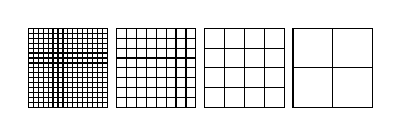
\begin{tikzpicture}
      [>=stealth,
      every node/.style={inner sep=2pt},
      restrict/.style={thick},
      prolong/.style={thick},
      mglevel/.style={rounded rectangle,draw=blue!50!black,fill=blue!20,thick,minimum size=4mm},
      ]
      \begin{scope}\scriptsize
        \newcommand\mgdx{4.0em}
        \newcommand\mgdy{4.0em}
        \newcommand\mgl[1]{(pow(2,#1+1))}
        \newcommand\mgloc[4]{(#1 + #4*\mgdx*#3,#2 + \mgdy*#3)}

        \newcommand\mghx{0.9*\mgdx}
        \newcommand\mghy{0.9*\mgdy}

        \draw[shift=\mgloc{0*\mgdx}{0}{0}{0},
        xstep=\mghy/\mgl{3},
        ystep=\mghy/\mgl{3}]
        (-0.5*\mghy,-0.5*\mghy) grid (0.5*\mghy,0.5*\mghy);

        \draw[shift=\mgloc{1*\mgdx}{0}{0}{0},
        xstep=\mghy/\mgl{2},
        ystep=\mghy/\mgl{2}]
        (-0.5*\mghy,-0.5*\mghy) grid (0.5*\mghy,0.5*\mghy);

        \draw[shift=\mgloc{2*\mgdx}{0}{0}{0},
        xstep=\mghy/\mgl{1},
        ystep=\mghy/\mgl{1}]
        (-0.5*\mghy,-0.5*\mghy) grid (0.5*\mghy,0.5*\mghy);


        \draw[shift=\mgloc{3*\mgdx}{0}{0}{0},
        xstep=\mghy/\mgl{0},
        ystep=\mghy/\mgl{0}]
        (-0.5*\mghy,-0.5*\mghy) grid (0.5*\mghy,0.5*\mghy);
      \end{scope}
    \end{tikzpicture}
    \label{fig:levels}
  \end{figure}
  \textbf{Multigrid} is an $O(n)$ method for solving algebraic problems by defining a hierarchy of scale.
  A multigrid method is constructed from:
  \begin{enumerate}
  \item a series of discretizations
    \begin{itemize}
    \item coarser approximations of the original problem
    \item constructed algebraically or geometrically
    \end{itemize}
  \item intergrid transfer operators
    \begin{itemize}
    \item residual restriction $I_h^H$ (fine to coarse)
    \item state restriction $\hat I_h^H$ (fine to coarse)
    \item partial state interpolation $I_H^h$ (coarse to fine, `prolongation')
    \item state reconstruction $\mathbb{I}_H^h$ (coarse to fine)
    \end{itemize}
  \item Smoothers ($S$)
    \begin{itemize}
    \item correct the high frequency error components
    \item Richardson, Jacobi, Gauss-Seidel, etc.
    \item Gauss-Seidel-Newton or optimization methods
    \end{itemize}
  \end{enumerate}
\end{frame}
\begin{frame}{$\tau$ formulation of Full Approximation Scheme (FAS)}
  \begin{itemize}
  \item classical formulation: ``coarse grid \emph{accelerates} fine grid solution''
  \item $\tau$ formulation: ``fine grid improves accuracy of coarse grid''
  \item To solve $N u = f$, recursively apply
    \begin{equation*}
      \begin{split}
        \text{pre-smooth} \:\: & \quad \tilde u^h \gets S^h_{\text{pre}}(u^h_0, f^h) \\
        \text{solve coarse problem for $u^H$} \:\: & \quad N^H u^H = f^H + \underbrace{N^H \hat I_h^H \tilde u^h - I_h^H N^h \tilde u^h}_{\tau_h^H} \\
        \text{correction and post-smooth} \:\: & \quad u^h \gets S^h_{\text{post}} \Big( \tilde u^h + I_H^h (u^H - \hat I_h^H \tilde u^h), f^h \Big) \\
      \end{split}
    \end{equation*}
    \begin{tabular}{ll}
      \toprule
      $I_h^H$ & residual restriction \\
      $\hat I_h^H$ & solution restriction \\
      $I_H^h$ & solution interpolation \\
      $f^H = I_h^H f^h$ & restriction of forcing term \\
      $\{S^h_{\text{pre}},S^h_{\text{post}}\}$ & smoothing operations on the fine grid \\
      \bottomrule
    \end{tabular}
  \end{itemize}
\end{frame}

\begin{frame}{Multiscale compression and recovery using $\tau$}
  % \begin{tikzpicture}
  %   [>=stealth,
  %   every node/.style={inner sep=2pt},
  %   restrict/.style={thick,double},
  %   prolong/.style={thick,double},
  %   cprestrict/.style={green!50!black,thick,double,dashed},
  %   control/.style={rectangle,red!40!black,draw=red!40!black,thick},
  %   mglevel/.style={rounded rectangle,draw=blue!50!black,fill=blue!20,thick,minimum size=4mm},
  %   checkpoint/.style={rectangle,draw=green!50!black,fill=green!20,thick,minimum size=4mm},
  %   mglevelhide/.style={rounded rectangle,draw=gray!50!black,fill=gray!20,thick,minimum size=4mm},
  %   tau/.style={text=red!50!black,draw=red!50!black,fill=red!10,inner sep=1pt}
  %   ]
  %   \begin{scope}\scriptsize
  %     \newcommand\mgdx{2.1em}
  %     \newcommand\mgdy{1.9em}
  %     \newcommand\mgloc[4]{(#1 + #4*\mgdx*#3,#2 + \mgdy*#3)}
  %     \node[mglevel] (fine0) at \mgloc{0}{0}{4}{-1} {\mglevelfine};
  %     \node[mglevel] (finem1down0) at \mgloc{0}{0}{3}{-1} {};
  %     \node[mglevel] (cp1down0) at \mgloc{0}{0}{2}{-1} {$\mglevelcp+1$};
  %     \node[mglevel] (cpdown0) at \mgloc{0}{0}{1}{-1} {\mglevelcp};
  %     \node[mglevel] (coarser0) at \mgloc{0}{0}{0}{0} {\ldots};

  %     \node[mglevelhide] (cpup0) at \mgloc{0}{0}{1}{1} {};
  %     \node (cp1up0) at \mgloc{0}{0}{2}{1} {};

  %     \node (cpdown1) at \mgloc{4em}{0}{1}{-1} {};
  %     \node[mglevelhide] (coarser1) at \mgloc{4em}{0}{0}{1} {\ldots};
  %     \node[mglevel] (cpup1) at \mgloc{4em}{0}{1}{1} {\mglevelcp};
  %     \node[mglevel] (cp1up1) at \mgloc{4em}{0}{2}{1} {$\mglevelcp+1$};
  %     \node[mglevel] (finem1up1) at \mgloc{4em}{0}{3}{1} {};
  %     \node[mglevel] (fine1) at \mgloc{4em}{0}{4}{1} {\mglevelfine};

  %     \draw[->,restrict,dashed] (fine0) -- (finem1down0);
  %     \draw[->,restrict] (finem1down0) -- (cp1down0);
  %     \draw[->,restrict] (cp1down0) -- (cpdown0);
  %     \draw[->,restrict,dashed] (cpdown0) -- (coarser0);
  %     \draw[->,prolong,dashed] (coarser0) -- (cpup0);
  %     \draw[->,prolong,dashed] (cpup0) -- (cp1up0);

  %     \draw[->,restrict,dashed] (cpdown1) -- (coarser1);
  %     \draw[->,prolong,dashed] (coarser1) -- (cpup1);
  %     \draw[->,prolong] (cpup1) -- (cp1up1);
  %     \draw[->,prolong] (cp1up1) -- (finem1up1);
  %     \draw[->,prolong,dashed] (finem1up1) -- (fine1);

  %     \node[checkpoint] at (4em + \mgdx*4,\mgdy) (cp) {CP};
  %     \draw[>->,cprestrict] (fine1) -- node[below,sloped] {Restrict} (cp);

  %     \node[left=\mgdx of fine0] (bnanchor) {};
  %     \node[control,fill=red!20] at (1.1*\mgdx,3*\mgdy) {Solve $F(u^n;b^n) = 0$};
  %     \node[mglevel,right=of fine1] (finedt) {next solve};
  %     \draw[->, >=stealth, control] (fine1) to[out=20,in=170] node[above] {$b^{n+1}(u^n,b^n)$} (finedt);
  %     \draw[->, >=stealth, control] (bnanchor) to[out=45,in=155] node[above] {$b^n$} (fine0);

  %     % Recovery process
  %     \begin{scope}[xshift=7*\mgdx]
  %       \node[checkpoint] (rcp) at \mgloc{0}{0}{0}{0} {CP};
  %       \node[mglevel] (r0a) at \mgloc{0}{\mgdy}{0}{0} {CR};
  %       \node[mglevel] (r1a) at \mgloc{0}{\mgdy}{1}{1} {};
  %       \node[mglevel] (r0b) at \mgloc{2*\mgdx}{\mgdy}{0}{0} {CR};
  %       \node[mglevel] (r1b) at \mgloc{2*\mgdx}{\mgdy}{1}{1} {};
  %       \node[mglevel] (r2b) at \mgloc{2*\mgdx}{\mgdy}{2}{1} {\mglevelfine};
  %       \node[mglevel] (r1c) at \mgloc{6*\mgdx}{\mgdy}{1}{-1} {};
  %       \node[mglevel] (r0d) at \mgloc{6*\mgdx}{\mgdy}{0}{0} {CR};
  %       \node[mglevel] (r1d) at \mgloc{6*\mgdx}{\mgdy}{1}{1} {};
  %       \node[mglevel] (r2d) at \mgloc{6*\mgdx}{\mgdy}{2}{1} {\mglevelfine};

  %       \draw[-,prolong,green!50!black] (rcp) -- (r0a);
  %       \draw[->,prolong] (r0a) -- (r1a);
  %       \draw[->,restrict] (r1a) -- (r0b);
  %       \draw[->,restrict] (r0b) -- (r1b);
  %       \draw[->,restrict,dashed] (r1b) -- (r2b);
  %       \draw[->,restrict,dashed] (r2b) -- (r1c);
  %       \draw[->,restrict] (r1c) -- (r0d);
  %       \draw[->,restrict] (r0d) -- (r1d);
  %       \draw[->,restrict,dashed] (r1d) -- (r2d);

  %       \foreach \smooth in {finem1down0, cp1down0, cpdown0, coarser0,
  %         cpup1, cp1up1, finem1up1,
  %         r0b,r1c,r0d,r1d} {
  %         \node[above left=-5pt of \smooth.west,tau] {$\tau$};
  %       }
  %       \node[rectangle,fill=none,draw=green!50!black,thick,fit=(rcp)(r2d)] (recoverbox) {};
  %       \node[rectangle,draw=green!50!black,fill=green!20,thick,minimum size=6mm,above={0cm of recoverbox.south east},anchor=south east] (recover) {FMG Recovery};
  %     \end{scope}
  %     \node (notation) at (-7.5*\mgdx,2*\mgdy) {
  %       \tiny
  %       \begin{minipage}{22em}\raggedright \sf
  %         $\bullet$ checkpoint converged coarse state \\
  %         $\bullet$ recover using FMG anchored at $\mglevelcp+1$ \\
  %         $\bullet$ compatible relaxation (CR) as coarse solve \\
  %         $\bullet$ $\tau$ correction is local, only $\mglevelcp$ neighbor points \\
  %         $\bullet$ survivors continue MG cycles with stale $\tau$
  %       \end{minipage}
  %     };
  %   \end{scope}
  % \end{tikzpicture}
  \includegraphics[width=\textwidth]{FMGRecovery}
    \begin{itemize}
    \item Compress transient simulation with local decompression
    \item Remove communication from all but coarse grid
      \begin{itemize}
      \item Convergence speed not affected, modest redundant computation
      \end{itemize}
    \item In-situ visualization and reanalysis with very few full checkpoints
    \item Checkpointing for discrete adjoints
    \item Resiliency to hardware failure
    \end{itemize}
\end{frame}


\begin{frame}{Model problem: $\pfrak$-Laplacian with slip boundary conditions}
  \begin{itemize}
  \item 2-dimensional model problem for power-law fluid cross-section
    \begin{equation*}
      -\div \big(\abs{\nabla u}^{\pfrak-2} \nabla u \big) - f = 0, \qquad 1 \le \pfrak \le \infty
    \end{equation*}
    Singular or degenerate when $\nabla u = 0$
  \item Regularized variant
    \begin{gather*}
      -\div (\eta \nabla u) - f = 0 \\
      \eta(\gamma) = (\epsilon^2 + \gamma)^{\frac{\pfrak-2}{2}} \qquad \gamma(u) = \half \abs{\nabla u}^2
    \end{gather*}
  \item Friction boundary condition on one side of domain
    \begin{gather*}
      \nabla u \cdot \bm n + A(x) \abs{u}^{q-1} u = 0
    \end{gather*}
  \end{itemize}
\end{frame}

\begin{frame}{Model problem: $\pfrak$-Laplacian with slip boundary conditions}
  \begin{itemize}
  \item $\pfrak = 1.3$ and $q = 0.2$, checkerboard coefficients $\{10^{-2},1\}$
  \item Friction coefficient $A=0$ in center, 1 at corners
  \end{itemize}
  \begin{columns}
    \begin{column}{0.5\textwidth}
      \only<1>{\includegraphics[width=\textwidth]{figures/MG/ex15-friction/visit0010.png}}
      \only<2>{\includegraphics[width=\textwidth]{figures/MG/ex15-friction/visit0011.png}}
      \only<3>{\includegraphics[width=\textwidth]{figures/MG/ex15-friction/visit0012.png}}
      \only<4>{\includegraphics[width=\textwidth]{figures/MG/ex15-friction/visit0013.png}}
      \only<5>{\includegraphics[width=\textwidth]{figures/MG/ex15-friction/visit0014.png}}
      \only<6>{\includegraphics[width=\textwidth]{figures/MG/ex15-friction/visit0015.png}}
    \end{column}
    \begin{column}{0.5\textwidth}
      \includegraphics[width=\textwidth]{figures/MG/newton-convergence.png}
    \end{column}
  \end{columns}
\end{frame}

\begin{frame}{$\tau$ corrections}
  \begin{figure}
  \centering
  \begin{subfigure}[b]{0.18\textwidth}
    \includegraphics[width=\textwidth]{figures/MG/ElasticityCompressTrim}
    %\caption{Initial solution.}\label{fig:elast-initial}
  \end{subfigure} ~
  \begin{subfigure}[b]{0.18\textwidth}
    \includegraphics[width=\textwidth]{figures/MG/ElasticityCompressShearTrim}
    %\caption{Increment.}\label{fig:elast-increment}
  \end{subfigure} ~
  \begin{subfigure}[b]{0.28\textwidth}
    \includegraphics[width=\textwidth]{figures/MG/ElasticityCompressErrorNoTauTrim}
    %\caption{Smoothed error without $\tau$.}\label{fig:elast-error-notau}
  \end{subfigure} ~
  \begin{subfigure}[b]{0.28\textwidth}
    \includegraphics[width=\textwidth]{figures/MG/ElasticityCompressErrorTauTrim}
    %\caption{Smoothed error with $\tau$.}\label{fig:elast-error-tau}
  \end{subfigure}
  \begin{itemize}
  \item Plane strain elasticity, $E=1000,\nu=0.4$ inclusions in $E=1,\nu=0.2$ material, coarsen by $3^2$.
  \item Solve initial problem everywhere and compute $\tau_h^H = A^H \hat I_h^H u^h - I_h^H A^h u^h$
  \item Change boundary conditions and solve FAS coarse problem
    \begin{equation*}
      N^H \acute u^H = \underbrace{I_h^H \acute f^h}_{\acute f^H} + \underbrace{N^H \hat I_h^H \tilde u^h - I_h^H N^h \tilde u^h}_{\tau_h^H}
    \end{equation*}
  \item Prolong, post-smooth, compute error $e^h = \acute u^h - (N^h)^{-1} \acute f^h$
  \item<2> \alert{Coarse grid \emph{with $\tau$} is nearly $10\times$ better accuracy}
  \end{itemize}
  % \caption{Plane strain elasticity, $E=1000,\nu=0.4$ inclusions in $E=1,\nu=0.2$ material.  2-level multigrid with coarsening factor of $3^2$.
  %   Panes (a) and (b) show the deformed body colored by strain.
  %   The initial problem of compression by 0.2 from the right is solved (a) and $\tau = A^H \hat I_h^H u^h - I_h^H A^h u^h$ is computed.
  %   Then a shear increment of 0.1 in the $y$ direction is added to the boundary condition, and the coarse-level problem is resolved, interpolated to the fine-grid, and a post-smoother is applied.
  %   When the coarse problem is solved without a $\tau$ correction (c), the displacement error is nearly $10\times$ larger than when $\tau$ is included in the right hand side of the coarse problem (d).
  % }\label{fig:tau-valid}
  % ./ex49 -mx 90 -my 90 -da_refine_x 3 -da_refine_y 3 -elas_ksp_converged_reason -elas_ksp_rtol 1e-8 -no_view -c_str 3 -sponge_E0 1 -sponge_E1 1e3 -sponge_nu0 0.4 -sponge_nu1 0.2 -sponge_t 3 -sponge_w 9 -u_o vtk:ex49_sol.vts -use_nonsymbc -elas_pc_type mg -elas_pc_mg_levels 2 -elas_pc_mg_galerkin -tau1_o vtk:ex49_tau1.vts -tau2_o vtk:ex49_tau2.vts -taudiff_o vtk:ex49_taudiff.vts -u2_o vtk:ex49_sol2.vts -u2c_o vtk:ex49_sol2c.vts -u3_o vtk:ex49_sol3.vts -u4_o vtk:ex49_sol4.vts -u2err_o vtk:ex49_sol2err.vts -u3err_o vtk:ex49_sol3err.vts -u3c_o vtk:ex49_sol3c.vts -tau3_o vtk:ex49_tau3.vts
\end{figure}
\end{frame}

\begin{frame}{$\tau$ adaptivity: an idea for heterogeneous media}
  \begin{itemize}
  \item Applications with localized nonlinearities
    \begin{itemize}
    \item Subduction, rifting, rupture/fault dynamics
    \item Carbon fiber, biological tissues, fracture
    \end{itemize}
  \item Adaptive methods fail for heterogeneous media
    \begin{itemize}
    \item Rocks are rough, solutions are not ``smooth''
    \item Cannot build accurate coarse space without scale separation
    \end{itemize}
  \item $\tau$ adaptivity
    \begin{itemize}
    \item Fine-grid work needed everywhere at first
    \item Then $\tau$ becomes accurate in nearly-linear regions
    \item Only visit fine grids in ``interesting'' places: active nonlinearity, drastic change of solution
    \end{itemize}
  \end{itemize}
\end{frame}

\begin{frame}{Comparison to nonlinear domain decomposition}
  \begin{itemize}
  \item ASPIN (Additive Schwarz preconditioned inexact Newton) \\
    \begin{itemize}
    \item Cai and Keyes (2003)
    \item More local iterations in strongly nonlinear regions
    \item Each nonlinear iteration only propagates information locally
    \item Many real nonlinearities are activated by long-range forces
      \begin{itemize}
      \item locking in granular media (gravel, granola)
      \item binding in steel fittings, crack propagation
      \end{itemize}
    \item Two-stage algorithm has different load balancing
      \begin{itemize}
      \item Nonlinear subdomain solves
      \item Global linear solve
      \end{itemize}
    \end{itemize}
  \item $\tau$ adaptivity
    \begin{itemize}
    \item Minimum effort to communicate long-range information
    \item Nonlinearity sees effects as accurate as with global fine-grid feedback
    \item Fine-grid work always proportional to ``interesting'' changes
    \end{itemize}
  \end{itemize}
\end{frame}

\begin{frame}{Low communication MG}
  \begin{columns}
    \begin{column}{0.55\textwidth}
      \begin{itemize}
      \item {\color{red} red arrows} can be removed by $\tau$-FAS with overlap
      \item {\color{blue} blue arrows} can also be removed, but then
        algebraic convergence stalls when discretization error is
        reached
      \item no simple way to check that discretization error is obtained
      \item if fine grid state is not stored, use compatible relaxation to complete prolongation $P$
      \end{itemize}
    \end{column}
    \begin{column}{0.45\textwidth}
      \vspace{-2em}
      \includegraphics[width=\textwidth]{figures/MG/LowCommunication}
    \end{column}
  \end{columns}
\end{frame}

\begin{frame}{Nonlinear problems}
  \begin{itemize}
  \item matrix-based smoothers require global linearization
  \item nonlinearity often more efficiently resolved locally
  \item nonlinear additive or multiplicative Schwarz
  \item nonlinear/matrix-free is good if
    \[ C = \frac{(\text{cost to evaluate residual at one point}) \cdot N}{(\text{cost of global residual})} \sim 1 \]
    \begin{itemize}
    \item finite difference: $C < 2$
    \item finite volume: $C \sim 2$, depends on reconstruction
    \item finite element: $C \sim \text{number of vertices per cell}$
    \end{itemize}
  \item larger block smoothers help reduce $C$
  \end{itemize}
  \vspace{-2.5em}
  \hfill \includegraphics[width=0.3\textwidth]{figures/NodeStencil}
\end{frame}


\begin{frame}[fragile]{Multiscale compression and recovery using $\tau$ form}
   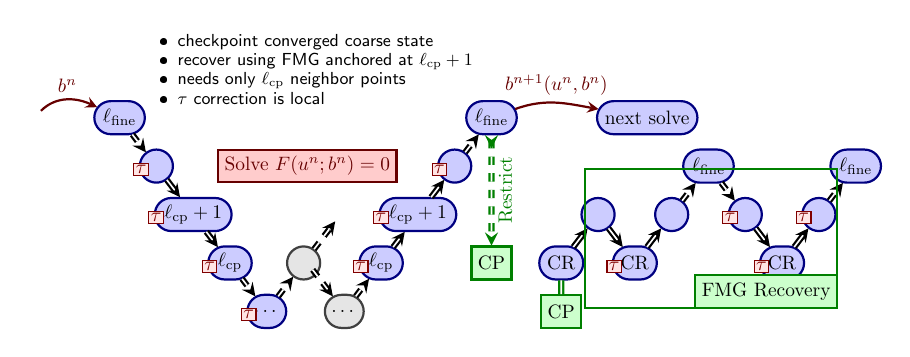
\begin{tikzpicture}
    [scale=0.7,every node/.style={scale=0.7},
    >=stealth,
    restrict/.style={thick,double},
    prolong/.style={thick,double},
    cprestrict/.style={green!50!black,thick,double,dashed},
    control/.style={rectangle,red!40!black,draw=red!40!black,thick},
    mglevel/.style={rounded rectangle,draw=blue!50!black,fill=blue!20,thick,minimum size=6mm},
    checkpoint/.style={rectangle,draw=green!50!black,fill=green!20,thick,minimum size=6mm},
    mglevelhide/.style={rounded rectangle,draw=gray!50!black,fill=gray!20,thick,minimum size=6mm},
    tau/.style={text=red!50!black,draw=red!50!black,fill=red!10,inner sep=1pt},
    crelax/.style={text=green!50!black,fill=green!10,inner sep=0pt}
    ]
    \begin{scope}
      \newcommand\mgdx{1.9em}
      \newcommand\mgdy{2.5em}
      \newcommand\mgloc[4]{(#1 + #4*\mgdx*#3,#2 + \mgdy*#3)}
      \node[mglevel] (fine0) at \mgloc{0}{0}{4}{-1} {\mglevelfine};
      \node[mglevel] (finem1down0) at \mgloc{0}{0}{3}{-1} {};
      \node[mglevel] (cp1down0) at \mgloc{0}{0}{2}{-1} {$\mglevelcp+1$};
      \node[mglevel] (cpdown0) at \mgloc{0}{0}{1}{-1} {\mglevelcp};
      \node[mglevel] (coarser0) at \mgloc{0}{0}{0}{0} {\ldots};

      \node[mglevelhide] (cpup0) at \mgloc{0}{0}{1}{1} {};
      \node (cp1up0) at \mgloc{0}{0}{2}{1} {};

      \node (cpdown1) at \mgloc{4em}{0}{1}{-1} {};
      \node[mglevelhide] (coarser1) at \mgloc{4em}{0}{0}{1} {\ldots};
      \node[mglevel] (cpup1) at \mgloc{4em}{0}{1}{1} {\mglevelcp};
      \node[mglevel] (cp1up1) at \mgloc{4em}{0}{2}{1} {$\mglevelcp+1$};
      \node[mglevel] (finem1up1) at \mgloc{4em}{0}{3}{1} {};
      \node[mglevel] (fine1) at \mgloc{4em}{0}{4}{1} {\mglevelfine};

      \draw[->,restrict,dashed] (fine0) -- (finem1down0);
      \draw[->,restrict] (finem1down0) -- (cp1down0);
      \draw[->,restrict] (cp1down0) -- (cpdown0);
      \draw[->,restrict,dashed] (cpdown0) -- (coarser0);
      \draw[->,prolong,dashed] (coarser0) -- (cpup0);
      \draw[->,prolong,dashed] (cpup0) -- (cp1up0);

      \draw[->,restrict,dashed] (cpdown1) -- (coarser1);
      \draw[->,prolong,dashed] (coarser1) -- (cpup1);
      \draw[->,prolong] (cpup1) -- (cp1up1);
      \draw[->,prolong] (cp1up1) -- (finem1up1);
      \draw[->,prolong,dashed] (finem1up1) -- (fine1);

      \node[checkpoint] at (4em + \mgdx*4,\mgdy) (cp) {CP};
      \draw[>->,cprestrict] (fine1) -- node[below,sloped] {Restrict} (cp);

      \node[left=\mgdx of fine0] (bnanchor) {};
      \node[control,fill=red!20] at (1.1*\mgdx,3*\mgdy) {Solve $F(u^n;b^n) = 0$};
      \node[mglevel,right=of fine1] (finedt) {next solve};
      \draw[->, >=stealth, control] (fine1) to[out=20,in=170] node[above] {$b^{n+1}(u^n,b^n)$} (finedt);
      \draw[->, >=stealth, control] (bnanchor) to[out=45,in=155] node[above] {$b^n$} (fine0);

      % Recovery process
      \begin{scope}[xshift=8*\mgdx]
        \node[checkpoint] (rcp) at \mgloc{0}{0}{0}{0} {CP};
        \node[mglevel] (r0a) at \mgloc{0}{\mgdy}{0}{0} {CR};
        \node[mglevel] (r1a) at \mgloc{0}{\mgdy}{1}{1} {};
        \node[mglevel] (r0b) at \mgloc{2*\mgdx}{\mgdy}{0}{0} {CR};
        \node[mglevel] (r1b) at \mgloc{2*\mgdx}{\mgdy}{1}{1} {};
        \node[mglevel] (r2b) at \mgloc{2*\mgdx}{\mgdy}{2}{1} {\mglevelfine};
        \node[mglevel] (r1c) at \mgloc{6*\mgdx}{\mgdy}{1}{-1} {};
        \node[mglevel] (r0d) at \mgloc{6*\mgdx}{\mgdy}{0}{0} {CR};
        \node[mglevel] (r1d) at \mgloc{6*\mgdx}{\mgdy}{1}{1} {};
        \node[mglevel] (r2d) at \mgloc{6*\mgdx}{\mgdy}{2}{1} {\mglevelfine};

        \draw[-,prolong,green!50!black] (rcp) -- (r0a);
        \draw[->,prolong] (r0a) -- (r1a);
        \draw[->,restrict] (r1a) -- (r0b);
        \draw[->,restrict] (r0b) -- (r1b);
        \draw[->,restrict,dashed] (r1b) -- (r2b);
        \draw[->,restrict,dashed] (r2b) -- (r1c);
        \draw[->,restrict] (r1c) -- (r0d);
        \draw[->,restrict] (r0d) -- (r1d);
        \draw[->,restrict,dashed] (r1d) -- (r2d);

        \foreach \smooth in {finem1down0, cp1down0, cpdown0, coarser0,
          cpup1, cp1up1, finem1up1,
          r0b,r1c,r0d,r1d} {
          \node[above left=-5pt of \smooth.west,tau] {$\tau$};
        }
        \node[rectangle,fill=none,draw=green!50!black,thick,fit=(rcp)(r2d)] (recoverbox) {};
        \node[rectangle,draw=green!50!black,fill=green!20,thick,minimum size=6mm,above={0cm of recoverbox.south east},anchor=south east] (recover) {FMG Recovery};
      \end{scope}
      \node (notation) at (\mgdx,5*\mgdy) {
        \begin{minipage}{18em}\small\sf
          \begin{itemize}\addtolength{\itemsep}{-5pt}
          \item checkpoint converged coarse state
          \item recover using FMG anchored at $\mglevelcp+1$
          \item needs only $\mglevelcp$ neighbor points
          \item $\tau$ correction is local
          \end{itemize}
        \end{minipage}
      };
    \end{scope}
  \end{tikzpicture}
  \begin{itemize}
  \item Normal multigrid cycles visit all levels moving from $n \to n+1$
  \item FMG recovery only accesses levels finer than $\ell_{CP}$
  % \item Only failed processes and neighbors participate in recovery
  \item Lightweight checkpointing for transient adjoint computation
  \item Postprocessing applications, e.g., in-situ visualization at high temporal resolution in part of the domain
  \end{itemize}
\end{frame}

\begin{frame}{Outlook on $\tau$-FAS adaptivity and compression}
  \begin{itemize}
  \item Benefits of AMR without fine-scale smoothness
  \item Coarse-centric restructuring is a major interface change
  \item Nonlinear smoothers (and discretizations)
    \begin{itemize}
    \item Smooth in neighborhood of ``interesting'' fine-scale features
    \item Which discretizations can provide efficient matrix-free smoothers?
    \item Does there exist an efficient smoother based on element Neumann problems?
    \end{itemize}
  \item Dynamic load balancing
  \item Reliability of error estimates for refreshing $\tau$
    \begin{itemize}
    \item We want a coarse indicator for whether $\tau$ needs to change
    \end{itemize}
  \item Worthwhile for resilience and to better use hardware
  \end{itemize}
\end{frame}

\end{document}
